\documentclass[11pt]{article}
\usepackage[utf8]{inputenc}
\usepackage[margin=1in]{geometry}
\usepackage{booktabs}
\usepackage{hyperref}
\usepackage{graphicx}

% \title{Design Review: Artix DC-SCM PCB Fabrication}
% \author{Fabian}
% \date{\today}

\begin{document}

% \maketitle


\section{BOM Obsolescence}
The following components are obsolete:
\begin{itemize}
    \item \textbf{DDR3 SDRAM:} Alliance AS4C256M16D3-12BIN. 
    \item \textbf{eMMC Flash:} Micron MTFC16GAPALNA-AIT-ND.
\end{itemize}

\section{PCB Fabrication \& DFM Blockers}
\begin{itemize}
    \item \textbf{Non-Standard Via Stackup:} Current design uses L1--L6 blind vias. This is asymmetrical for an 8-layer board and requires expensive sequential lamination. Or it can't be manufactured by most manufacturers.

    \item \textbf{Unoptimized DRC Rules:} The Default Design constraints are messy(figure \ref{fig:design-constrains}). For example 0mm clearance between Tracks. After i changed those values to minimum values of different manufacturers there are some DRC Errors. (Example \ref{fig:weirdtrace}) 

    \item Different Stackup in Fabrication Files, Website and in the Kicad setup: I checked the impedances for the different stackups and only the impedance in the fabrication file leads to the correct impedance. 

    \item Unnecessary restrictive constrains makes the design not well suited for Manufacturability which is why most manufacturers are not able to manufacture the board. 

\end{itemize}

\begin{figure}[h]
  \centering
  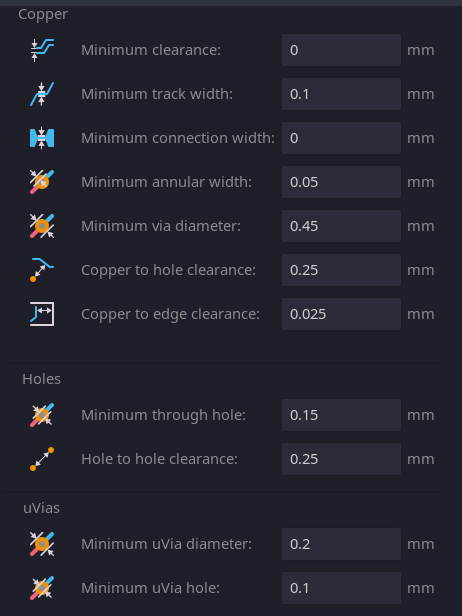
\includegraphics[width=0.8\textwidth]{img/Design Constrains.png}
  \caption{}
  \label{fig:design-constrains}
\end{figure}


\begin{figure}[h]
  \centering
  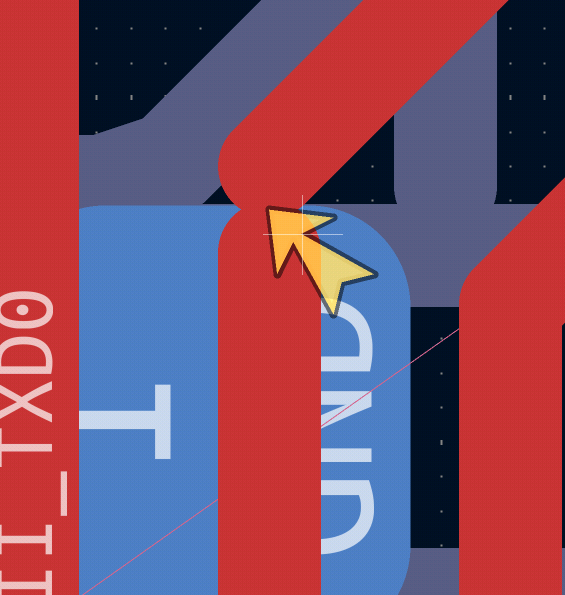
\includegraphics[width=0.8\textwidth]{img/WeirdTrace.png}
  \caption{}
  \label{fig:weirdtrace}
\end{figure}

\section{Impedance Issues}

Impedances are matched using Online Calculators. Kicads Internal tool leads to different Impedance values. Online Calculators are not sufficient for small traces and spacing!!

\section{Before Ordering}
\begin{itemize}
  \item Check Minor DRC Errors
  \item Try to get rid of 1-6 vias and replace them with through hole vias.
  \item Choose one manufacturer and change the traces to have the right impedance for their stackup
  \item Check Impedances \textbf{Impedance Control}: Factory changes the traces based on their parameters.
\end{itemize}

\section{PCB Manufacturers}
Since there are so hard constrains i had to search for many different manufacturers and see if they are able to manufacture the board. So far i checked the following ones. For the prices i calculated 5 boards since it is the minimum for many assembly houses.
\begin{itemize}
  \item \textbf{PCBWay}: I requested a quote from them to have a baseline for the price. They are able to manufacture any layer HDI boards. For 5 boards: \$758.53(Without tax) + 
\$ 1656.37 for assembly including the parts
  \item \textbf{Eurocircuit}: Can't manufacture 1-6 vias for 8 layer board. Also no via stacking. Without those vias: € 3538.92 (Only so expensive because of hard constrains)
  \item \textbf{Wuerth Electronics}1-6 via not possible for their normal stackups. € 1.320,75	with less strict constrains
  \item \textbf{Multi-CB} Should be capable of creating the PCB but has no assembly service. Since This is a really custom stackup i had to request manually and still have no reply. (706.52 € for only one pcb)
  \item \textbf{Leiton}Should be capable of creating the PCB and assemble but since this is a really special request this is only done manually and i have no reply yet.
\end{itemize}


\section{Modification Estimate: 32x IO Integration}
Should be doable. This (figure \ref{fig:areaasic}) has some space that should be enough to route the traces to the asic depending on the footprint size. If there is not enough space I have to move some footprints and do most of the routing again. Since the FPGA has a relatively large pitch maybe it would be better to do the routing again and optimize for Manufacturability.

Check IO voltages


\begin{figure}[h]
  \centering
  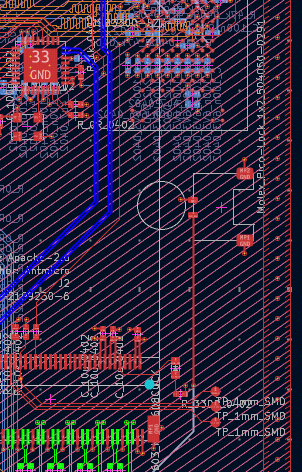
\includegraphics[width=0.8\textwidth]{img/AreaAsic.png}
  \caption{}
  \label{fig:areaasic}
\end{figure}

\section{Impedance Control Requirements}
\begin{center}
\begin{tabular}{l l l}
\toprule
\textbf{Interface} & \textbf{Signal Type} & \textbf{Target Impedance} \\
\midrule
PCIe Gen 2 & Differential Pairs & 85$\Omega \pm 10\%$ \\
Ethernet (Media) & Differential Pairs & 100$\Omega \pm 10\%$ \\
RGMII (MAC side) & Single-Ended & 50$\Omega \pm 10\%$ \\
USB & Differential & 90$\Omega \pm 15\%$ \\
\bottomrule
\end{tabular}
\end{center}

\section{DDR3}

Generally, single impedances (CA, Control \& DQ’s) are 50Ω (+/- 10\%) 
and differential impedances (Clocks, DQS’s) are nominally 100Ω (+/- 10\%) and are typically routed on inner layers if 
possible.
\\

The following are general guidelines for PDN development in DDR3 board designs. 
\begin{itemize}
\item1. Solid Power and Ground planes should be used in DDR3 routing areas. 
\item2. Place a 0.1uF cap and 0.01uF as close as possible for every VDDQ pin. 
\item3. VTT decoupling should be as close to the components and pull-up resistors as possible. 
\item4. Place a 0.1uF decoupling cap between VTT and VDD. 
\item5. Low ESL decoupling capacitors should be used, and routing should be carefully evaluated to minimize 
inductance. 
\item 6. Power connections from supply planes to vias for device pins or decoupling capacitors should be as short ($<$8 
mils) and as wide as possible (trace widths should be the same or larger than the via size) to minimize trace 
impedance. 
\end{itemize}

\section{changed}

- changed ddr3\_clk\_p with ddr3\_a9 (easier routing)
- changed ddr3\_clk\_n with ddr3\_a5

\end{document}
